\documentclass[12pt, a4paper]{article}

%% Text related
\usepackage[utf8]{inputenc}
\usepackage{indentfirst}
\usepackage[bottom]{footmisc}
\usepackage{verbatim} %Adds comment blocks & code copy-paste
\usepackage[ngerman, num]{isodate} %Proper date format ffs...
    \monthyearsepgerman{}{}
    \daymonthsepgerman{}{}
\usepackage{enumitem}
\usepackage{lipsum} %Because why not?
\usepackage{lscape}

%% Figure related
\usepackage{graphicx}
\usepackage{float} 
\usepackage{subfig}
\usepackage[justification=centering]{caption} %Centers multiline captions

%% Drawing stuff
\usepackage{pgfplots}
\usepackage[american]{circuitikz}

%% Math & Scientific notations
\usepackage{amsmath}
\usepackage{amssymb} %amsmath doesn't have quite common math symbols for some reason
\usepackage[per-mode=repeated-symbol, tight-spacing=true]{siunitx}

%% Table related
\usepackage{multirow}
\usepackage{tabularx}
\usepackage[thinlines]{easytable} %convenient
\usepackage{booktabs} %for different horizontal lines
\usepackage{array} %for table corners not meeting up - doesn't appear to work though

%%
\usepackage{subfiles}

% pgfplots configurations
\graphicspath{ {../img/} }
\pgfplotsset{
    compat=newest,
    standard/.style={
    axis x line=middle,
    axis y line=middle,
    every axis x label/.style={at={(current axis.right of origin)},anchor=west},
    every axis y label/.style={at={(current axis.above origin)},anchor=south}
    }
}

% To place e.g. [ V ] so I don't bother typing it
\newcommand{\unitV}{{\;[\,\SI{}{\volt}\,]}}
\newcommand{\unitmA}{{\;[\,\SI{}{\milli\ampere}\,]}}
\newcommand{\unitA}{{\;[\,\SI{}{\ampere}\,]}}
\newcommand{\unitohm}{{\;[\,\SI{}{\ohm}\,]}}
\newcommand{\unitkohm}{{\;[\,\SI{}{\kilo\ohm}\,]}}

% \title{EED 3009 ENGINEERING DESIGN - II\\FEASIBILITY REPORT}
% \author{Abdurrahman ÜZÜM}
% \date{\today}




\begin{document}

    \begin{titlepage}
        \begin{center}

            \begin{figure}

                \subfloat
                {%
                    
\includegraphics[width=0.3\textwidth]{deulogo.png}
                }
                %
                \hfill
                %
                \subfloat
                {%
                    
\includegraphics[width=0.3\textwidth]{facultylogo.png}
                }

            \end{figure}

            \textbf{T.C.\\}
            \textbf{DOKUZ EYLUL UNIVERSITY\\}
            \textbf{ENGINEERING FACULTY\\}

            \vspace*{1 cm}
            \textbf{ELECTRICAL \& ELECTRONICS ENGINEERING\\}
            \textbf{DEPARTMENT\\}

            \vspace*{1 cm}
            \textbf{EED3009 ENGINEERING DESIGN - II\\}
            \textbf{THEORETICAL DESIGN REPORT\\}

            \textbf{RANGE FINDER}

            \vspace*{1 cm}

        
            \begin{table}[H]\centering
                \begin{tabular}{cc}
                    Elif Sezin ÖZYİĞİT \hspace{1cm}  & \hspace{1cm} Abdurrahman ÜZÜM \\
                    2019502098         \hspace{1cm}  & \hspace{1cm} 2019502099       \\             
                \end{tabular}
            \end{table}

            Instructor:\\ Dr.Ogr.Uy.Neslihan AVCU\\

            \vspace*{1 cm}
            December, 2022


        \end{center}

    \end{titlepage}

    \pagebreak
    
    \tableofcontents

    \pagebreak

    \begin{abstract}
        Early societies measured distance with a variety of primitive tools, from basic paces to measuring rods and marked ropes.\cite{abstract} Luckily, we’ve come a long way from the days of using belts, thumbs and cubits for measurement. Various methods have been developed over the years in order to increase the measurement accuracy and to be able to measure in various conditions. These devices, which have been developed by human beings step by step over the years and evolved with new technologies, have reached the level where they can measure without the need for physical contact or even light.
    \end{abstract}

    \section{Introduction}

        This project focuses on measuring distances with no contact up to a meter. To realise this project a battery powered, handheld device will be designed. The device will utilise an ultrasonic speaker and microphone. It will send regular periodic ultrasonic bursts from the speaker and listen for the echoes. The necessary circuitry will measure the time between sent ultrasonic bursts and their respective echoes, following the time of flight (ToF) principle. This data will then be processed using necessary information such as the speed of sound on air, as a result of which, the distance data will be obtained. Finally, this distance value will be printed on a two digit display. The device will also employ a laser guide to assist proper alignment of the sensors, and also to provide a feedback to the user. 


    \section{Objectives of the Project}

        \noindent The designed device must follow the above guidelines and accomplish these aims. 
        \begin{itemize}
            \item Measure distances in the range of 0-99\SI{}{\centi\metre}
            \item Have an accuracy of \SI{1}{\centi\metre}
            \item Be battery powered and handheld
            \item Display the measured distance in real time on a two digit display.
            \item Not empoly an MCU or ASIC designed for this particular purpuse.
        \end{itemize}

        \noindent In terms of measurement accuracy and range, the given properties can evolve as the experiments and tests continue, and therefore are subject to change. 

        
    \pagebreak
    \section{Overview of the Project}

        \begin{figure}[H]\centering
            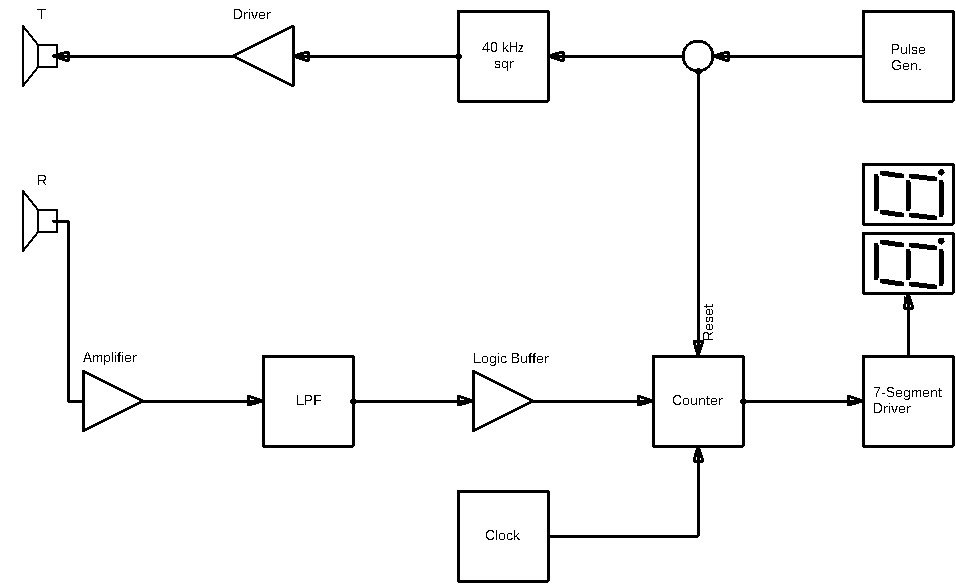
\includegraphics[width = \textwidth]{schematics/blockdiagram_v3.png}
            \caption[]{Revised Block Diagram}
        \end{figure}

        \bigskip
        Guidelines of distance measurement using ultrasonic sensors is relatively straight forward. All the device should do is to send sound signals, wait for the echoes arrive and measure the time between. Since transmitting a continuous signal would produce a continuous echo, it is not possible to keep track of the time. Therefore the transmitter should emit bursts of sound waves, and the receiver should keep track of the time between.

        \bigskip 
        Two ultrasonic transducers are needed, one for the transmitter and one for the receiver. The transmitter should be driven periodically with short pulses. The timing between these pulses is critical, such that the following pulse should not be transmitted before the echo of the previous pulse has arrived. This calculation should be made in consideration of the longest distance to be measured. Width of these pulses is also critical, as it should be short enough to ensure that the echo doesn't arrive before the pulse ends. This calculation should be made in considetation of the shortest distance of interest. 
    

    \pagebreak    
    \section{Design and Methodology}
    	\subsection{Ultrasonic Frequency Synthesis}
	
	Synthesizing sinusoidal waves is rather involved and hard. This is usually done digitally by the help of microcontrollers. Since this project does not allow the use of microcontrollers, and there are no readily available sinusoidal signal generator IC’s, it has been decided that driving the transmitter with square waves will suffice. This is also how the HCSR04 module was operating. Refer to the feasibility report Section 4 Figure 5 .
	
	\bigskip
	It is better to drive the transducer via a symmetrical wave, in order to use full swing range of the device. However, since the circuit will be powered via a 9V battery, there won’t be a negative rail. To accomplish this, H BRIDGE EXPLANATION
	
	\subsection{Burst Generation}
	Since transmitting a continuous signal would produce a continuous echo, it is not possible to keep track of the time. Therefore the transmitter should emit bursts of sound waves, and the receiver should keep track of the time between.

To accomplish this, another 555 can be used in astable mode with adjustable duty cycle.
	
	\subsection{Transmitter Driver}
	After obtaining the power requirements of the transmitter, a separate driver IC may be concluded to be necessary. In such case, a simple power amplifier / audio opamp can be used to deliver the necessary power to the transmitter. This driver should be selected such that it is able to operate at the ultrasonic frequencies without distortion. Since the transmitter is driven via two separate timer circuits, two power amplifiers are needed. 
	
	\subsection{Receiver Amplifier}
	During the transmission of the signal, it gets weaker. Since the received signal will be small in amplitude, in order to compensate this loss, it must be amplified to be used in the following blocks.
	
	\subsection{Low Pass Filter}
	Since the incoming echo signal will be a frequency modulated signal, where it consists of an ultrasonic burst filling a pulse, in order to obtain the actual waveform, it is necessary to pass the signal through a low pass filter. After this stage, the ultrasonic part will be discarded and following stages will see only the outlining pulse. This LPF can be a simple passive RC LPF.
	
	A passive first order RC low pass filter is designed with corner frequency fc ~= 5kHz. Where input signal consists of a 40kHz carrier and 150 Hz \%0.3 duty pulses. Passing this signal through a LPF enables it to be further passed though a schmitt trigger and recover the digital pulse, resulting in clean fast rising and falling edges, sufficient to trigger the counter.

To encounter attenuation, a schottky diode is placed to prevent capacitor to be discharged over lower value programming resistor, whose value is fixed to get necessary corner frequency. Instead, a bigger bleeder resistor is added in parallel with the capacitor. This allows output signal to rise relatively quickly though the LPF resistor, during “on” times of the input signal, and prevents it discharge though the same resistor during “off” times, and therefore decrease the inevitable attenuation, increasing the voltage level sufficient enough to drive the input of 5V logic schmitt trigger.
	
	\subsection{Low Pass Filter}
	After the LPF, even though the signal will resemble a pulse, it still will be an analogue signal, with slow rising/falling edges and an ambiguous amplitude value. To digitise the signal, it can be fed through a logical schmitt-trigger, output of which will be a truly digital signal. This can be accomplished using generic schmitt-trigger IC such as 74HC14.

	Even though the amplitude value does contain information about surface type and angle, these informations are beyond the scope of this project and therefore can be discarded without any problems in this stage.
	
	\subsection{Counter}
	
	\subsection{Display Driver}
	After obtaining a binary representation of distance at the output of the counter, this should be translated in an apropriate with which the 7-segment displays can  be driven. This can be accomplished by means of using a generic “binary to 7-segment” display driver IC such as 74HC4543.
	
    
   \pagebreak
    Assuming that the longest distance to be measured is \SI{100}{\centi\metre}, and speed of sound is \SI{343}{\metre\per\second}, the echo would arrive after:

    \begin{equation}
        \texttt{max }t_f = 2 \times \frac{\SI{1}{\metre}}{\SI{343}{\metre\per\second}} = \SI{5.83}{\milli\second}
    \end{equation}

    \noindent Therefore the time between end of a pulse and start of the other should be around \SI{6}{\milli\second} minimum. 

    \noindent Assuming that the shortest distance to be measured is \SI{1}{\centi\metre}, 

    \begin{equation}
        \texttt{min }t_f = 2 \times \frac{\SI{0.01}{\metre}}{\SI{343}{\metre\per\second}} = \SI{58.3}{\micro\second}
    \end{equation}

    \noindent Therefore the width of the pulse should not exceed about \SI{50}{\micro\second}.


    \bigskip
    Commonly available cheap ultrasonic transducers work at frequencies near \SI{40}{\kilo\hertz}. Therefore the transmitter should send bursts of \SI{40}{\kilo\hertz} sound waves, filling in the previously described pulse. In order to provide a signal with these properties, two generators are needed. One to generate the \SI{40}{\kilo\hertz} signal, and another to generate the pulses. The \SI{40}{\kilo\hertz} signal should then be connected to the transmitter via an analogue switch, which is driven by the pulses.
    
    \bigskip
    On the receiver side, the received signal will most likely be very low in amplitude, therefore the first stage is to amplify it. This amplification should be made such that the lowest possible echo should not fall short of the limits of the next stage, and the highest possible amplitude echo should not exceed it.
    
    \bigskip
    After the amplification, the \SI{40}{\kilo\hertz} sound burst should be converted into a regular pulse with digital voltage levels. To accomplish this, firstly the signal should be passed though a lowpass filter with appropriate passband frequency. After which, the signal will resemble a single pulse, albeit with slow-rising edges. Feeding this signal into a logical buffer/schmitt-trigger, the pulse can be converted into a true digital pulse. 

    \bigskip
    After converting the echo burst into a digital pulse, timing measurements can be done. A counter that is to be started simultaneously with the first edge of the transmitted burst, should then be stopped by the first edge of the echo signal. Output of the counter is proportional to the distance, however, it is necessary to convert it into proper units. For which an arithmetic circuit should follow the counter.

    \bigskip
    After obtaining the meaningful distance data, it then can be transferred to the 7-segment displays. A binary to 7 segment display driver can be employed here for simplicity.


    \pagebreak

    \section{Results}
    
    
        \pagebreak
            
    \section{Needs of the Project / BOMList}

      
    \pagebreak
     \section{Discussion}
     
      \pagebreak
     \section{Conclusion}
     
     \pagebreak
    \section{Gannt Chart}

        \begin{figure}[H]\centering
            \makebox[\linewidth]
                {
                    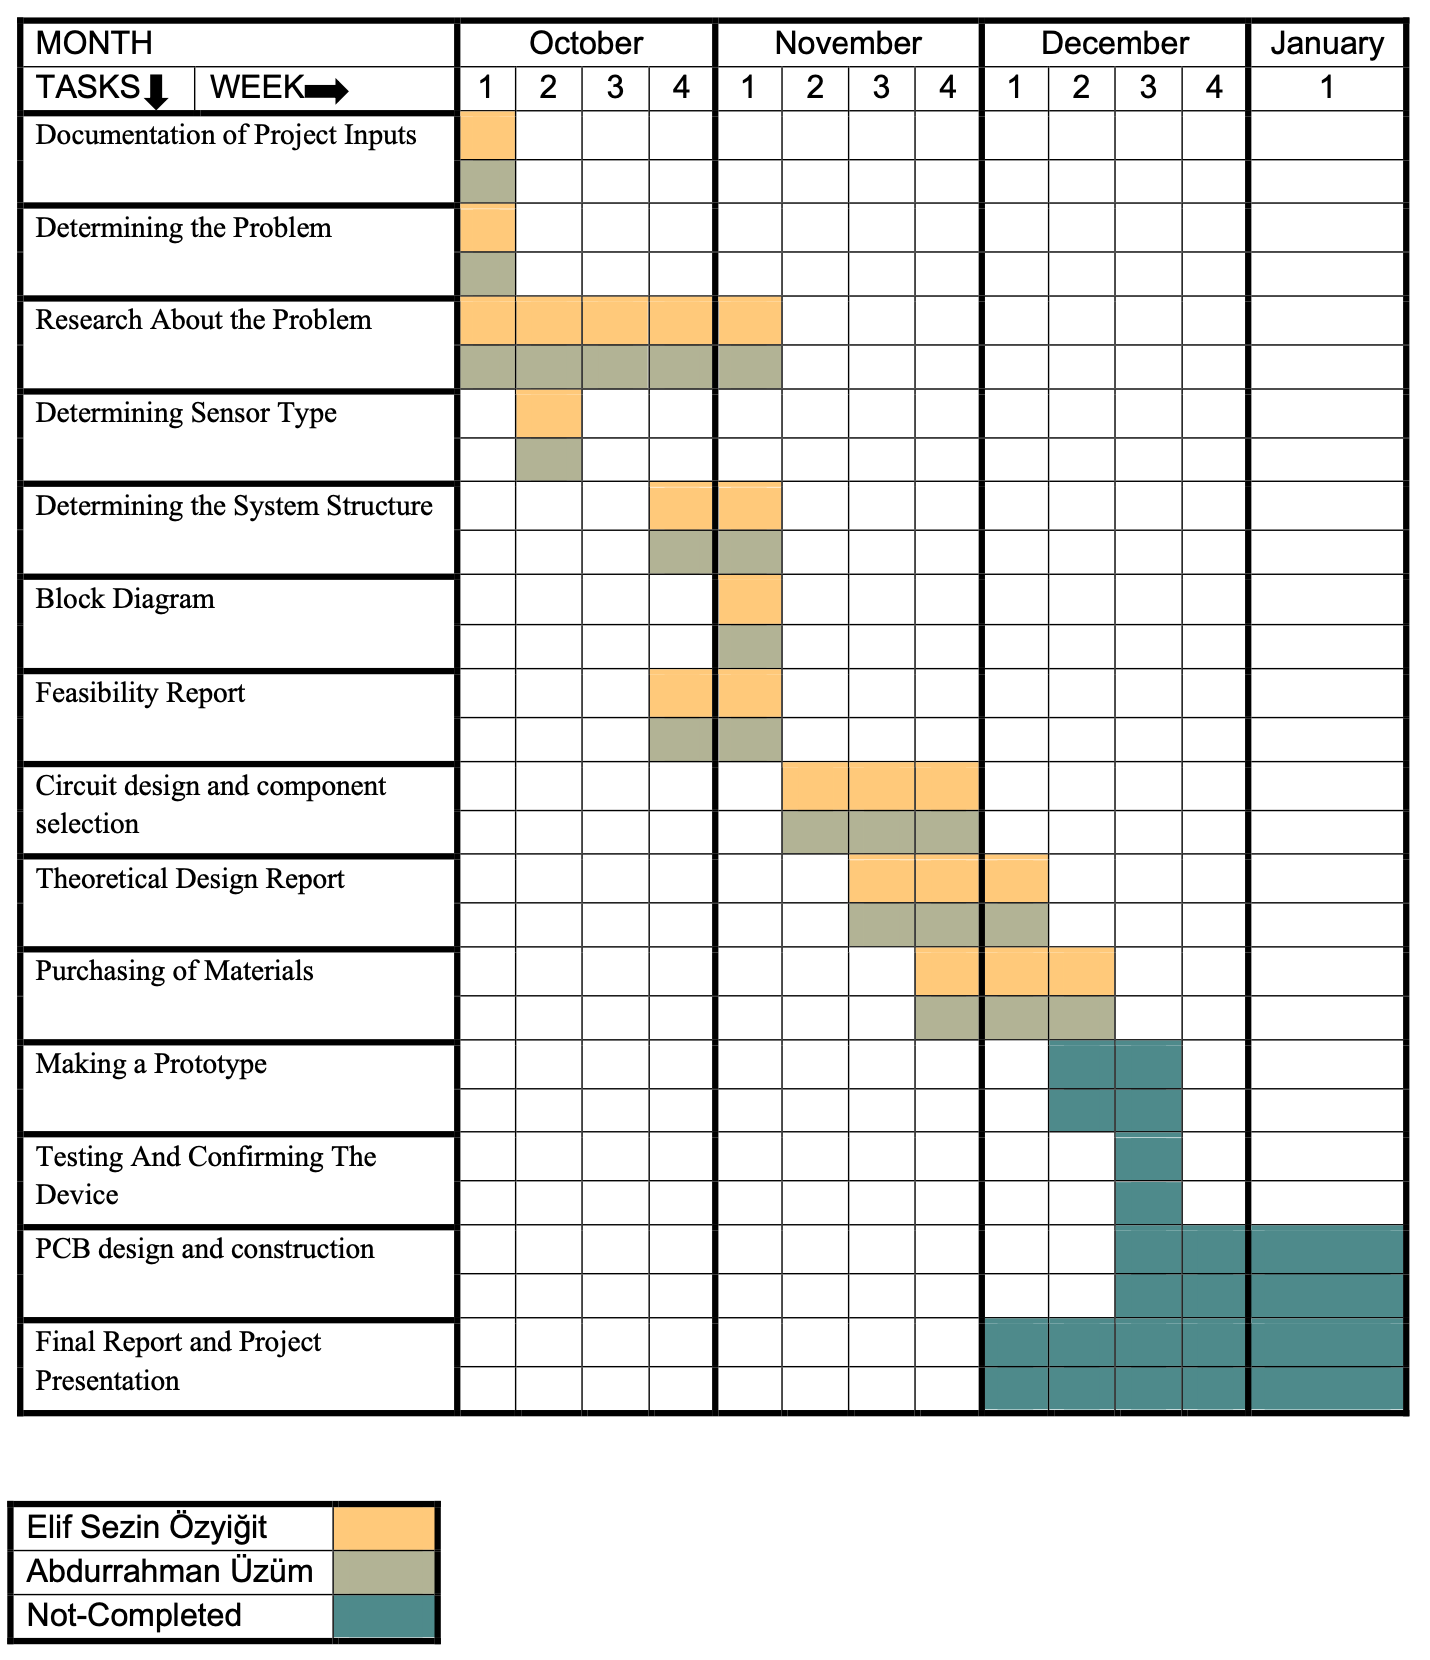
\includegraphics[width=1.2\linewidth]{Gantt_Chart_v2.png}
                }
                \caption{Gannt Chart}
        \end{figure}



    


    \begin{thebibliography}{}	
        \bibitem{abstract}
        https://www.encyclopedia.com/education/news-wires-white-papers-and-books/distance-measurement

        \bibitem{triangulation}
        https://www.seeedstudio.com/blog/2019/12/23/distance-sensors-types-and-selection-guide/

        \bibitem{tof}
        https://www.sensorpartners.com/en/knowledge-base/everything-about-the-operation-principles-of-ultrasonic-sensors/ 
        
        \bibitem{}
        \textit{Mubina Toa, Akeem Whitehead}, \textbf{\textit{``Ultrasonic Sensing Basics''}}, Texas Instruments
    \end{thebibliography}
            





\end{document}